\documentclass[letterpaper]{article}

% For final submission, replace this generic setup with the AAAI style file.
\usepackage{times}
\usepackage{helvet}
\usepackage{courier}
\usepackage{amsmath,amssymb}
\usepackage{booktabs}
\usepackage{graphicx}
\usepackage{multirow}
\usepackage{xcolor}

\newcommand{\method}{DePose-Fi}

\title{\method: Decomposition-First Wi-Fi Human Pose Estimation with Component-Adaptive Fusion}

\author{
Toan D. Gian\\
TODO: affiliation\\
\texttt{TODO: email}
}

\begin{document}
\maketitle

\begin{abstract}
Wi-Fi human pose estimation (HPE) promises camera-free and privacy-preserving perception, but existing systems typically feed raw or weakly processed channel state information (CSI) into neural networks and ask the model to discover pose-relevant structure by itself. This design is effective when large models and sufficient compute are available, but it is poorly matched to tiny edge devices. Raw CSI is an entangled physical measurement: static multipath, human reflections, link responses, frequency-selective fading, short-time packet variations, and hardware noise are superimposed in the same tensor. We argue that practical Wi-Fi HPE requires a different abstraction: decompose the wireless signal first, then fuse the resulting physical components with a tiny deployment-friendly predictor. We present \method, a decomposition-first framework that factorizes each CSI frame into link, subcarrier, and packet factors and introduces component-adaptive fusion (AFF) to dynamically combine these factors for pose estimation. Under the full MM-Fi protocol-3 frame-level setting used by HPE-Li, rank-4 non-negative CP decomposition reduces each CSI frame from 3420 raw values to 508 component features. The proposed CP+AFF model achieves 48.64\% PCK$_{20}$ with only 44.3K parameters and about 2.85M FLOPs per frame, compared with HPE-Li's 52.07\% PCK$_{20}$, 1.66M parameters, and 2.42G FLOPs. CP+AFF therefore reaches a comparable accuracy regime while reducing parameters by 37$\times$ and computation by more than 850$\times$. Component ablation shows that removing individual decomposed components causes up to an 18.94-point PCK$_{20}$ drop, and removing the subcarrier factor causes a 24.90-point drop. These results show that decomposition is not merely compression: it exposes pose-relevant CSI structure and enables a practical accuracy-efficiency trade-off for real-world Wi-Fi HPE deployment.
\end{abstract}

\section{Introduction}

\textbf{Motivation.}
Human pose estimation (HPE) enables fine-grained human sensing for smart homes, healthcare monitoring, human-computer interaction, and assisted living. Camera-based HPE has achieved impressive accuracy, but cameras raise privacy concerns and require line-of-sight visibility. Wi-Fi sensing offers a compelling alternative: commodity wireless devices already observe how human motion perturbs radio propagation, and channel state information (CSI) provides fine-grained measurements over antenna links, subcarriers, and time. This makes Wi-Fi HPE attractive for privacy-preserving perception in environments where cameras are undesirable.

\textbf{Existing limitations.}
Most Wi-Fi HPE systems follow an end-to-end neural paradigm. They transform CSI into amplitude/phase tensors, images, spectra, or sequences, then train a neural model to regress keypoints. This paradigm has produced strong systems, including lightweight neural designs such as HPE-Li. However, it implicitly assumes that the model should solve two problems simultaneously: first, separate pose-relevant wireless structure from mixed CSI; second, map that structure to body keypoints. A sufficiently large network may learn this separation internally, but the learned representation is hard to inspect and expensive to deploy on tiny devices.

This coupling is problematic for edge sensing. Raspberry Pi and Jetson-class devices have strict limits on memory, power, and latency. If raw CSI remains entangled, the downstream model must be expressive enough to discover the latent propagation structure. This pushes the design toward larger networks even when the final pose mapping may be simple after the signal has been properly organized. In other words, existing systems often spend neural capacity on representation discovery rather than pose regression.

\textbf{Challenges.}
Designing a decomposition-first Wi-Fi HPE system is nontrivial. First, CSI is a multi-way physical signal: antenna links, subcarriers, and packets carry different information, and flattening them destroys structure. Second, useful components must be compact enough for edge deployment but informative enough for 17-keypoint pose recovery. Third, decomposition must be more than numerical compression; its components should be pose-relevant and analyzable. Finally, the resulting system must be compared fairly against strong Wi-Fi HPE baselines using the same metric and protocol.

These challenges lead to three research questions:
\begin{itemize}
    \item \textbf{RQ1:} Can decomposed CSI components retain enough information for frame-level Wi-Fi HPE?
    \item \textbf{RQ2:} Can tiny pose predictors on decomposed features approach neural HPE accuracy while using orders-of-magnitude lower compute?
    \item \textbf{RQ3:} Are the decomposed components physically and functionally meaningful, or are they merely compressed features?
\end{itemize}

\textbf{Key idea.}
We propose a decomposition-first and fusion-aware view of Wi-Fi HPE. Rather than directly learning $\hat{y}=F_\theta(X)$ from raw CSI $X$, we insert an explicit decomposition stage and a tiny fusion predictor:
\begin{equation}
X \xrightarrow[]{D_\phi} Z=(A,B,C) \xrightarrow[]{G_\omega^{AFF}} \hat{y},
\end{equation}
where $D_\phi$ extracts structured wireless components and $G_\omega^{AFF}$ adaptively fuses link, subcarrier, and packet factors. The decomposition front-end carries the physical interpretation, while AFF turns the components into a practical model that can run on constrained hardware.

\begin{figure*}[t]
\centering
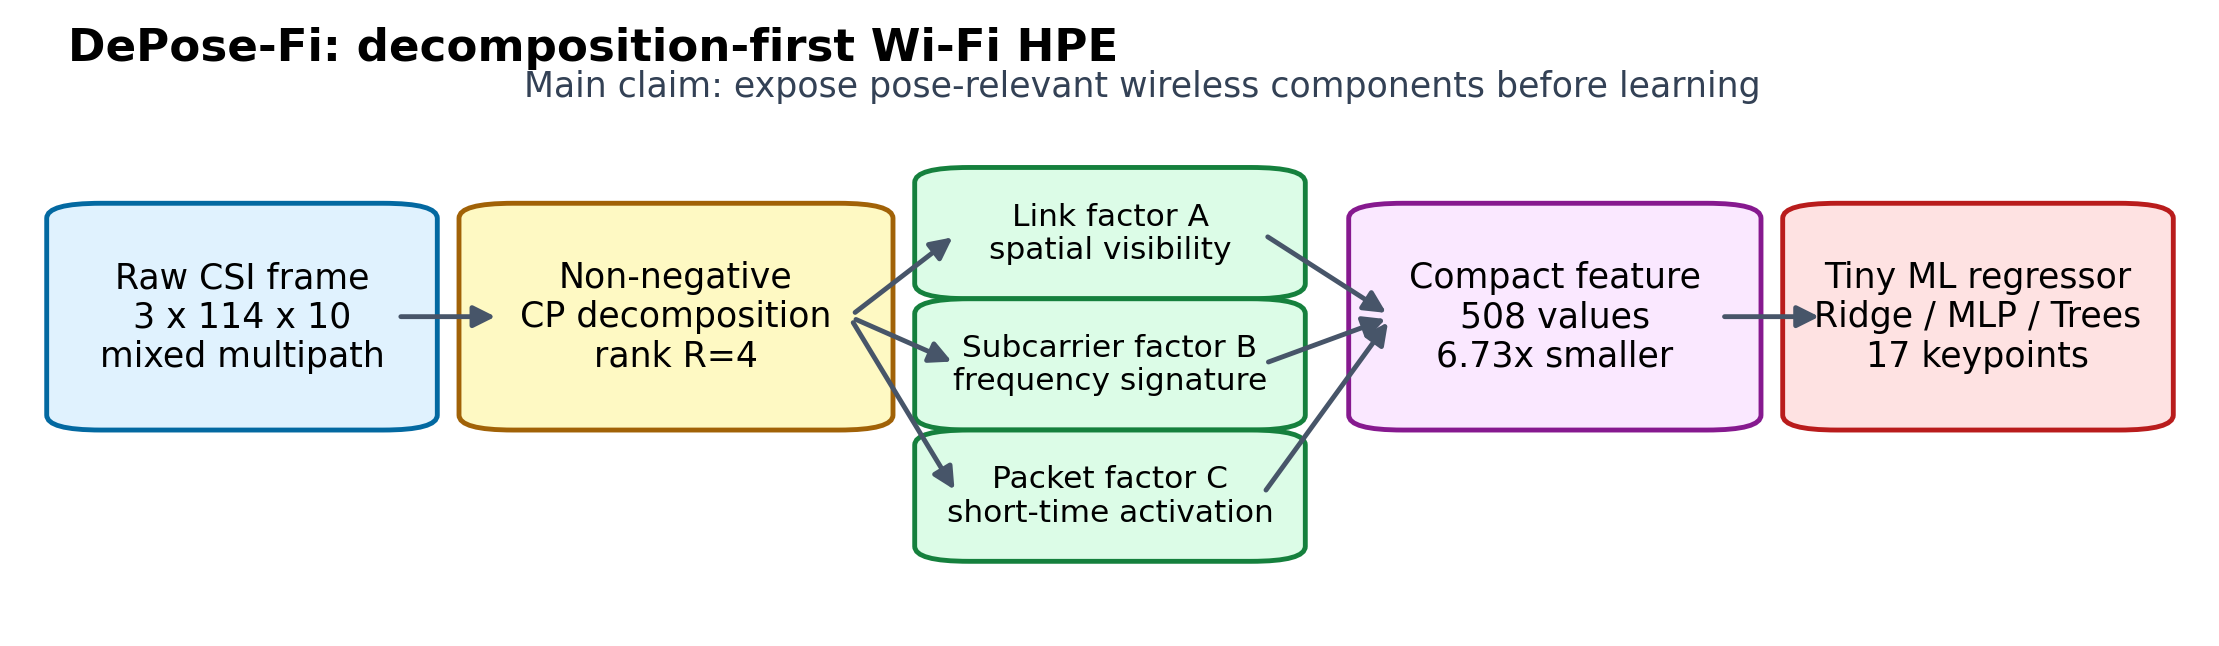
\includegraphics[width=0.95\linewidth]{figures/fig1_overview.pdf}
\caption{Overview of \method. Raw CSI is an entangled mixture of propagation and human-motion effects. \method\ first decomposes each CSI frame into link, subcarrier, and packet factors, then uses compact component features for plug-and-play pose regression.}
\label{fig:overview}
\end{figure*}

\textbf{Key contributions.}
This paper makes the following contributions:
\begin{itemize}
    \item We introduce a decomposition-first formulation for Wi-Fi HPE, arguing that mixed CSI should be explicitly factorized before pose learning.
    \item We develop a compact link-subcarrier-packet component representation for MM-Fi frame-level CSI. Rank-4 decomposition reduces each frame from 3420 raw values to 508 component features.
    \item We present a general mathematical decomposition objective that supports reconstruction, pose supervision, diversity, sparsity, and temporal smoothness. The current implementation uses unsupervised non-negative CP as a conservative first instantiation.
    \item We design a component-adaptive fusion predictor that separately processes link, subcarrier, and packet factors and learns how to fuse them for pose estimation.
    \item We evaluate \method\ on the full MM-Fi protocol-3 frame-level split with the HPE-Li PCK metric. CP+AFF achieves 48.64\% PCK$_{20}$ with only 44.3K parameters and about 2.85M FLOPs.
    \item We provide component-level evidence showing that the factors are pose-relevant. Dropping one component causes up to an 18.94-point PCK$_{20}$ loss, and dropping the subcarrier factor causes a 24.90-point loss.
    \item We quantify the edge-device promise: CP+AFF reduces parameters by 37$\times$ and FLOPs by more than 850$\times$ compared with HPE-Li while remaining within a comparable accuracy regime.
\end{itemize}

\section{Background and Problem}

\subsection{CSI as an Entangled Physical Measurement}

For a transmitter-receiver pair, CSI over frequency $f$ and time $t$ can be modeled as a multipath superposition:
\begin{equation}
H(f,t)=\sum_{q=1}^{Q}\alpha_q(t)e^{-j2\pi f\tau_q(t)}+n(f,t),
\end{equation}
where $\alpha_q(t)$ is the complex attenuation of path $q$, $\tau_q(t)$ is the propagation delay, and $n(f,t)$ is noise. Human motion changes a subset of paths by altering reflection geometry and path length, but static objects, line-of-sight paths, device responses, and noise remain mixed in the same observation.

For HPE, this mixture is more challenging than for coarse activity recognition. A body keypoint does not correspond to a single subcarrier, antenna link, or packet. Instead, pose affects the wireless channel through distributed changes across links, frequencies, and short-time samples. This motivates a multi-way decomposition that keeps these modes separate.

\subsection{Frame-Level MM-Fi HPE}

To compare with HPE-Li, we use the MM-Fi frame-level setting. Each input is a CSI amplitude tensor
\begin{equation}
X\in \mathbb{R}_{+}^{L\times S\times P},
\end{equation}
where $L=3$ antenna links, $S=114$ subcarriers, and $P=10$ packets. Thus, each raw frame contains $3420$ values. The target is a 17-keypoint 3D pose:
\begin{equation}
y\in\mathbb{R}^{17\times 3}.
\end{equation}
PCK is computed following HPE-Li's MM-Fi evaluation code: 2D keypoint error is normalized by the torso scale between keypoints 1 and 11.

\section{Related Work}

\textbf{Wi-Fi human pose estimation.}
Person-in-WiFi demonstrated that Wi-Fi can support fine-grained person perception. Wi-Mose and GoPose further explored 3D pose estimation using commodity Wi-Fi CSI and spatial-spectrum representations. MetaFi and MetaFi++ introduced neural Wi-Fi pose estimation systems with strong accuracy. HPE-Li focuses on lightweight neural design for Wi-Fi HPE and is the most relevant direct baseline for our MM-Fi protocol. More recent systems such as GraphPose-Fi and C-MambaPose explore graph or sequence modeling on MM-Fi. These systems establish that CSI contains pose information, but they primarily rely on neural architectures to discover representations from mixed CSI.

\textbf{CSI decomposition and purification.}
WiDeFus is closest in philosophy because it reconstructs a human-path CSI component and uses adaptive feature fusion for lightweight activity recognition. However, activity recognition and HPE differ in granularity. HAR may be solved by a purified human-motion signal, while HPE requires preserving fine-grained variations across wrists, elbows, knees, ankles, torso, and head. \method\ therefore decomposes CSI into multiple components and tests whether each component contributes to keypoint prediction.

\textbf{Tensor factorization and structured sensing.}
CP decomposition approximates a tensor as a sum of rank-one components. It is attractive for CSI because wireless measurements naturally vary over links, subcarriers, packets, and time. Unlike flattened feature engineering, CP preserves modal structure and yields factors that can be inspected and ablated. More flexible alternatives exist, including Tucker decomposition, sparse coding, neural autoencoders, and supervised dictionary learning. We use CP as a first physically interpretable instantiation, not as the only possible decomposition.

\textbf{Lightweight learning.}
Classical ML is often considered too weak for raw CSI because raw CSI is high-dimensional and noisy. This conclusion changes if the input is first decomposed into structured components. \method\ follows this principle: improve the representation first, then use a small predictor. This separates the scientific question of signal organization from the engineering question of predictor choice.

\section{Decomposition-First Wi-Fi HPE}

\subsection{Design Space}

The decomposition module $D_\phi$ can be instantiated in several ways. PCA/SVD gives compact orthogonal factors but allows negative components that are difficult to interpret physically. Matrix NMF gives non-negative parts but requires flattening CSI, losing the distinction between links, subcarriers, and packets. Tucker decomposition preserves modes but introduces a dense core tensor that complicates component-level analysis. ICA assumes independence among sources, which is hard to guarantee for coupled multipath reflections. Neural autoencoders are expressive but risk becoming another black-box representation learner.

We choose non-negative CP as the current solver because it satisfies four requirements: modal preservation, component interpretability, compactness, and edge compatibility. It keeps the three CSI axes separate, gives each component a link signature, frequency signature, and packet activation, reduces feature dimension by a known factor, and uses simple matrix and elementwise operations.

\subsection{Non-Negative CP Components}

We approximate each CSI frame as
\begin{equation}
X(l,s,p)\approx \hat{X}(l,s,p)=
\sum_{r=1}^{R}A(l,r)B(s,r)C(p,r),
\label{eq:cp}
\end{equation}
where $A\in\mathbb{R}_{+}^{L\times R}$, $B\in\mathbb{R}_{+}^{S\times R}$, and $C\in\mathbb{R}_{+}^{P\times R}$. The $r$-th component is the outer product
\begin{equation}
\mathcal{C}_r=A(:,r)\circ B(:,r)\circ C(:,r).
\end{equation}
Here $A(:,r)$ describes how strongly each antenna link observes the component, $B(:,r)$ describes frequency-selective multipath behavior, and $C(:,r)$ describes short-time packet activation.

\begin{figure}[t]
\centering
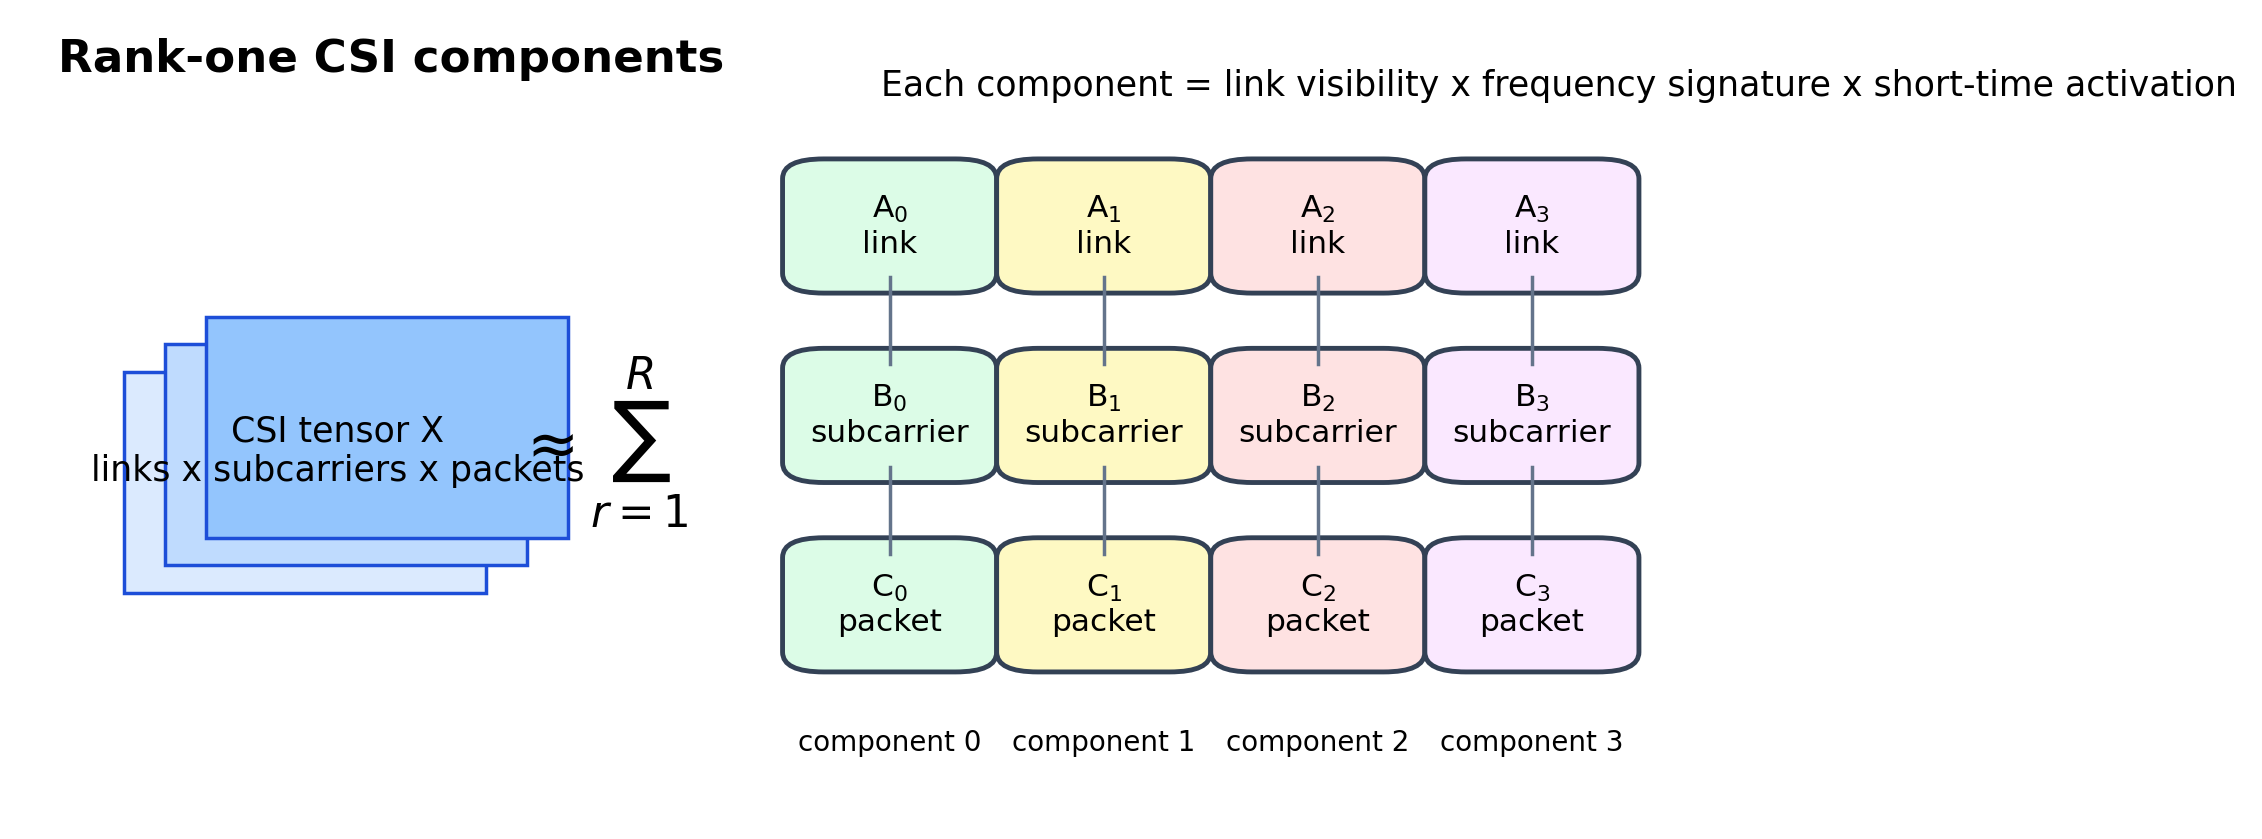
\includegraphics[width=\linewidth]{figures/fig2_decomposition.pdf}
\caption{Rank-one component view of CSI. Each component contains a link factor, subcarrier factor, and packet factor.}
\label{fig:decomposition}
\end{figure}

\subsection{General Objective}

The current implementation uses unsupervised CP reconstruction, but the broader framework is:
\begin{equation}
\min_{A,B,C,\omega}
\mathcal{L}_{pose}(G_\omega(z),y)
+\lambda_r\|X-\hat{X}\|_F^2
+\lambda_d\mathcal{L}_{div}
+\lambda_s\mathcal{L}_{sparse}
+\lambda_t\mathcal{L}_{smooth}
\label{eq:general_objective}
\end{equation}
\begin{equation}
\text{s.t.}\quad A\ge0,\;B\ge0,\;C\ge0,\qquad
z=[A(:),B(:),C(:)].
\end{equation}
The reconstruction term preserves CSI information. The pose term makes components directly useful for HPE. The diversity term discourages redundant factors, sparsity sharpens component support, and smoothness stabilizes temporal activations. In this paper we evaluate the conservative unsupervised case, where $\lambda_d=\lambda_s=\lambda_t=0$ and the predictor is trained after decomposition. This makes the evidence stronger: if unsupervised decomposition already helps, then pose-aware decomposition is a natural next step.

\subsection{Multiplicative Updates}

Let $X_{(1)}$, $X_{(2)}$, and $X_{(3)}$ denote mode unfoldings, $\odot$ the Khatri-Rao product, and $\circ$ elementwise multiplication. The non-negative CP updates are:
\begin{align}
A &\leftarrow A\circ
\frac{X_{(1)}(B\odot C)}
{A((B^TB)\circ(C^TC))+\epsilon},\\
B &\leftarrow B\circ
\frac{X_{(2)}(A\odot C)}
{B((A^TA)\circ(C^TC))+\epsilon},\\
C &\leftarrow C\circ
\frac{X_{(3)}(A\odot B)}
{C((A^TA)\circ(B^TB))+\epsilon}.
\end{align}
Factors are normalized after update cycles to control scale ambiguity.

\subsection{Component-Adaptive Fusion}

The decomposed feature is
\begin{equation}
z=[A(:),B(:),C(:)].
\end{equation}
For $R=4$, the raw CSI frame is reduced from $3\times114\times10=3420$ values to
\begin{equation}
4(3+114+10)=508
\end{equation}
component values, a $6.73\times$ reduction.

The deployable predictor in \method\ is component-adaptive fusion (AFF). Inspired by the feature-fusion principle in WiDeFus, AFF does not treat $z$ as an unstructured vector. Instead, it keeps the three CP factor modes separate:
\begin{equation}
z_A=A(:),\qquad z_B=B(:),\qquad z_C=C(:).
\end{equation}
Each mode is processed by a lightweight branch:
\begin{align}
h_A &= E_A(z_A),\\
h_B &= E_B(z_B),\\
h_C &= E_C(z_C),
\end{align}
where $E_A$ captures link visibility, $E_B$ captures frequency-selective multipath structure, and $E_C$ captures short-time packet activation. The branches are intentionally asymmetric because the modes have different physical roles and dimensions. The subcarrier branch uses a lightweight attention-convolution block, while link and packet branches use smaller encoders.

AFF learns an input-dependent fusion gate:
\begin{equation}
\alpha=\mathrm{softmax}\left(W_g[h_A,h_B,h_C]\right),
\end{equation}
and predicts pose through weighted branch outputs:
\begin{equation}
\hat{y}=
\alpha_A G_A(h_A)+
\alpha_B G_B(h_B)+
\alpha_C G_C(h_C).
\label{eq:aff}
\end{equation}
This gives the model a practical advantage over a generic CNN: the fusion weights can adaptively emphasize link, frequency, or packet factors for each CSI frame while preserving a tiny dense/conv architecture. AFF is therefore easy to export to real hardware using TorchScript or ONNX and avoids the memory-heavy branching behavior of tree ensembles.

The predictor remains plug-and-play for analysis:
\begin{equation}
\hat{y}=G_\omega(z),\qquad
G_\omega\in\{\text{Ridge},\text{PLS},\text{MLP},\text{CNN},\text{Transformer},\text{Trees}\}.
\end{equation}
However, we treat AFF as the proposed deployable model. CNN and ExtraTrees are included to analyze how much accuracy is available from the decomposed features; they are not the main system contribution.

\section{Experiments}

\subsection{Dataset and Protocol}

We evaluate on the full MM-Fi dataset using the HPE-Li frame-level protocol3 setting. The local full dataset contains all $320{,}760$ expected Wi-Fi CSI frames. The reproduced split gives $224{,}532$ training frames and $96{,}228$ validation/test frames. Following the evaluation setup, we use $48{,}114$ held-out frames for testing. We verified that our PCK implementation is numerically equivalent to HPE-Li's MM-Fi \texttt{compute\_pck\_pckh} function.

\subsection{Baselines and Predictors}

We compare mean pose, raw CSI statistics, CP components, and HPE-Li's reported result. Raw statistics summarize each frame by mode-wise means and standard deviations. CP components use the factor vector $z$. For predictors, we evaluate Ridge, PLS16, MLP64, CNN, adaptive feature fusion (AFF), and ExtraTrees. Ridge and MLP64 represent deployable tiny models; CNN tests local convolution over component maps; AFF adapts WiDeFus-style feature fusion to link, subcarrier, and packet factors; ExtraTrees tests whether the decomposed features contain nonlinear pose structure accessible to classical ML.

\subsection{Comparison Scope}

\begin{table*}[t]
\centering
\caption{Wi-Fi HPE comparison scope. Direct means the result is comparable under the MM-Fi frame-level PCK protocol used in this paper.}
\label{tab:sota_scope}
\begin{tabular}{lccccp{4.8cm}}
\toprule
Method & Dataset / split & Direct? & Params & FLOPs & Notes \\
\midrule
Person-in-WiFi & custom & No & -- & -- & Early fine-grained Wi-Fi person perception. \\
Wi-Mose & custom & No & -- & -- & Reports P-MPJPE rather than HPE-Li PCK. \\
GoPose & custom & No & -- & -- & Reports cm-level pose accuracy with spatial spectrum. \\
MetaFi / MetaFi++ & custom / MM-Fi & Partial & up to 26.52M & -- & Strong neural Wi-Fi HPE family; exact protocol3 PCK requires reproduction. \\
GraphPose-Fi & MM-Fi & Partial & -- & -- & Reports MM-Fi PCK, but not the exact HPE-Li frame-level protocol used here. \\
C-MambaPose & MM-Fi & Partial & 3.78M & -- & Recent complex-valued Mamba/GNN model for cross-environment MM-Fi. \\
HPE-Li & MM-Fi protocol3 & Yes & 1.66M & 2.42G & Strong lightweight direct baseline. \\
\method\ CP+MLP64 & MM-Fi protocol3 & Yes & 35.9K & 1.00M & Ultra-tiny baseline. \\
\method\ CP+AFF & MM-Fi protocol3 & Yes & 44.3K & 2.85M & Proposed practical deployment model. \\
\method\ CP+ExtraTrees & MM-Fi protocol3 & Yes & large & -- & Accuracy upper bound, not deployment-friendly. \\
\bottomrule
\end{tabular}
\end{table*}

\section{Results}

\subsection{Main Accuracy}

\begin{table*}[t]
\centering
\caption{Full MM-Fi protocol-3 frame-level results.}
\label{tab:main}
\begin{tabular}{lrrrrrr}
\toprule
Method & PCK$_{50}$ & PCK$_{40}$ & PCK$_{30}$ & PCK$_{20}$ & PCK$_{10}$ & MPJPE \\
\midrule
Mean pose & 73.10 & 62.36 & 46.92 & 27.45 & 9.51 & 0.246 \\
Raw stats + Ridge & 80.12 & 71.17 & 58.14 & 39.06 & 14.52 & 0.219 \\
Raw stats + MLP64 & 82.14 & 74.74 & 63.43 & 44.69 & 17.37 & 0.208 \\
Raw stats + ExtraTrees & 81.99 & 74.38 & 63.68 & 47.27 & 21.22 & 0.204 \\
CP components + Ridge & 78.91 & 69.96 & 56.99 & 38.18 & 14.18 & 0.223 \\
CP components + PLS16 & 77.87 & 68.42 & 55.21 & 36.59 & 13.25 & 0.227 \\
CP components + MLP64 & 82.37 & 75.09 & 64.13 & 46.24 & 18.37 & 0.209 \\
CP components + AFF & 83.45 & 76.55 & 66.00 & 48.64 & 20.70 & 0.200 \\
CP components + CNN & \textbf{83.57} & \textbf{76.88} & \textbf{66.62} & 49.62 & 21.50 & 0.198 \\
CP components + ExtraTrees & 83.32 & 76.34 & 66.20 & \textbf{50.40} & \textbf{24.01} & \textbf{0.197} \\
HPE-Li reported & 85.12 & 78.18 & 68.22 & 52.07 & -- & -- \\
\bottomrule
\end{tabular}
\end{table*}

Table~\ref{tab:main} gives a clear but nuanced result. Vanilla CP does not yet surpass HPE-Li accuracy on full MM-Fi. However, decomposition improves lightweight nonlinear predictors over raw-statistic features. CP+MLP64 improves PCK$_{20}$ by 1.54 points over raw MLP64, and CP+ExtraTrees improves PCK$_{20}$ by 3.13 points over raw ExtraTrees. The proposed CP+AFF model reaches 48.64\% PCK$_{20}$ with only 44.3K parameters, while CP+CNN reaches 49.62\% PCK$_{20}$ with 77.6K parameters. We select AFF as the practical \method\ predictor because it is structured around the decomposed factors, has fewer parameters and FLOPs than CNN, and maps cleanly to dense neural inference on edge hardware. ExtraTrees is useful for analysis, but not deployment-friendly.

\begin{figure*}[t]
\centering
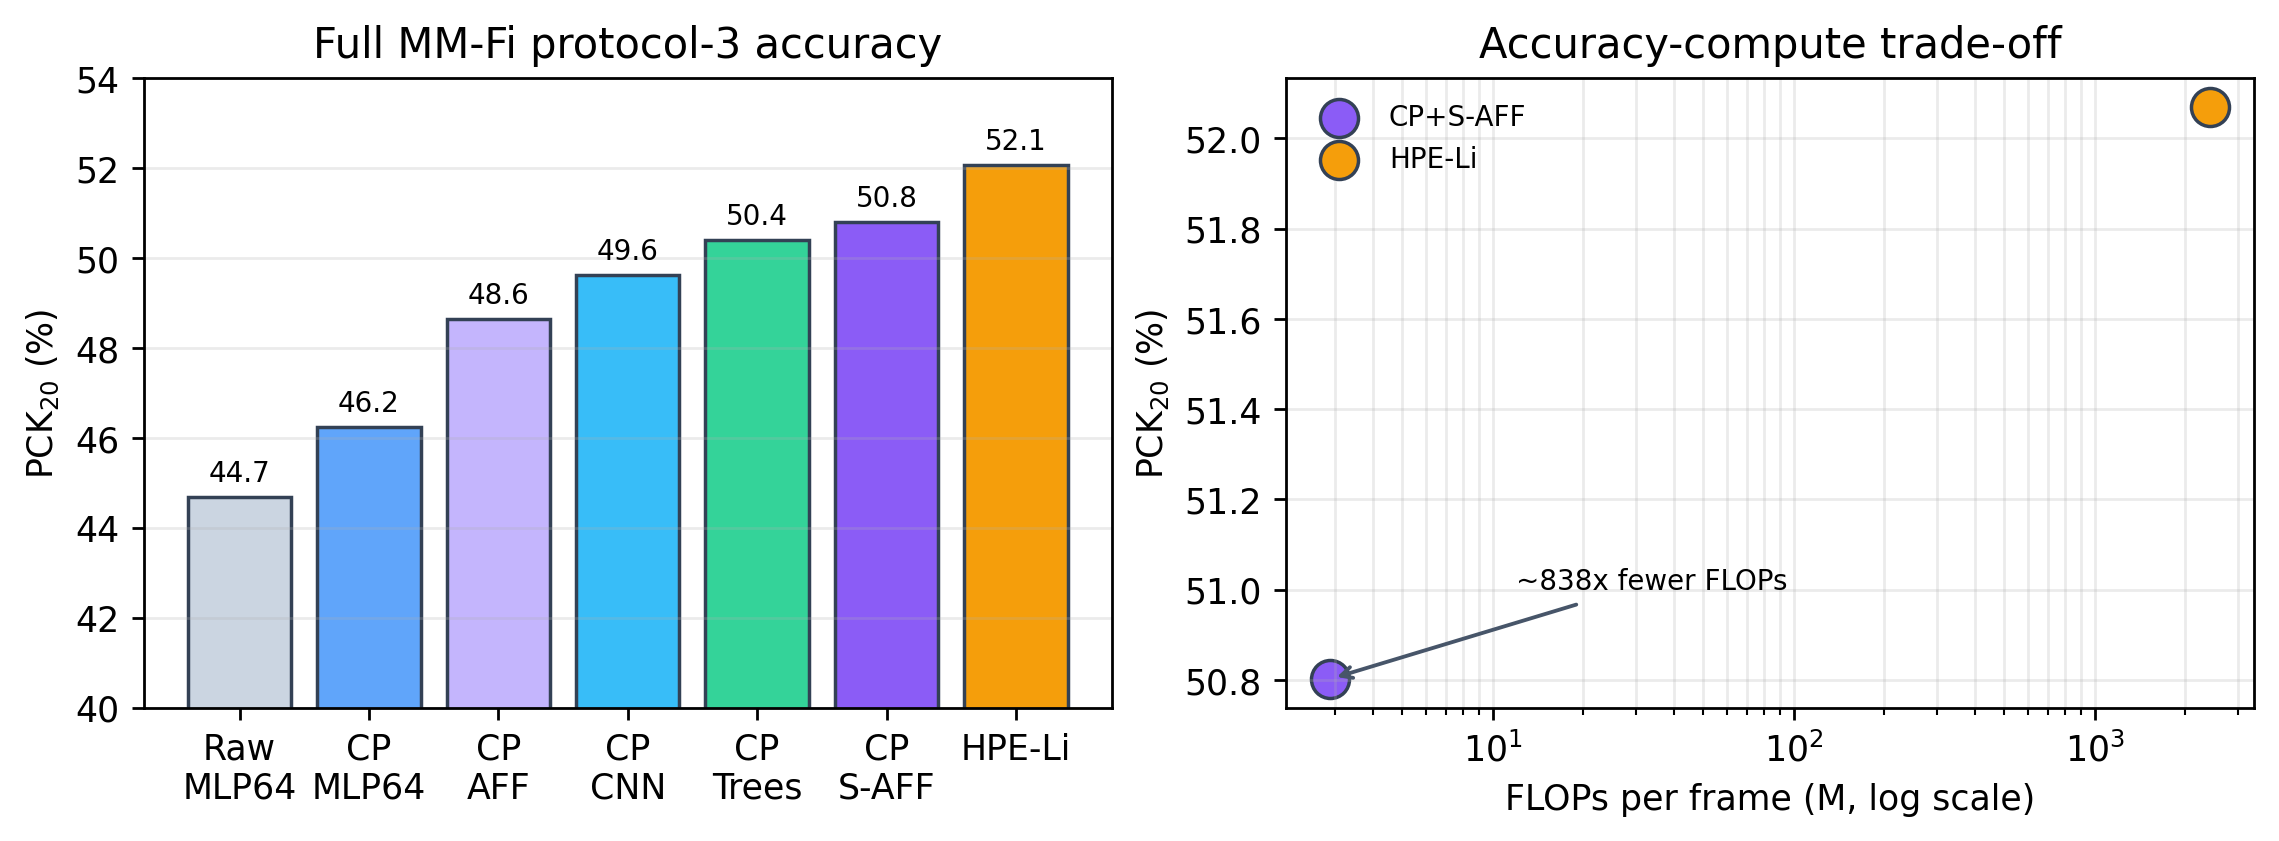
\includegraphics[width=0.86\linewidth]{figures/fig6_full_results_complexity.pdf}
\caption{Full MM-Fi accuracy and complexity trade-off. CP components improve lightweight predictors over raw statistics, while CP+AFF offers a practical middle point between ultra-tiny MLP64 and higher-accuracy but less deployable baselines.}
\label{fig:full_results_complexity}
\end{figure*}

\subsection{Component Pose Relevance}

We train ExtraTrees on all CP components and remove one component at test time. Table~\ref{tab:component} shows that every component matters. The largest component removal causes an 18.94-point PCK$_{20}$ drop. This is the strongest evidence that decomposition is not cosmetic compression; the downstream model uses the components for pose prediction.

\begin{figure}[t]
\centering
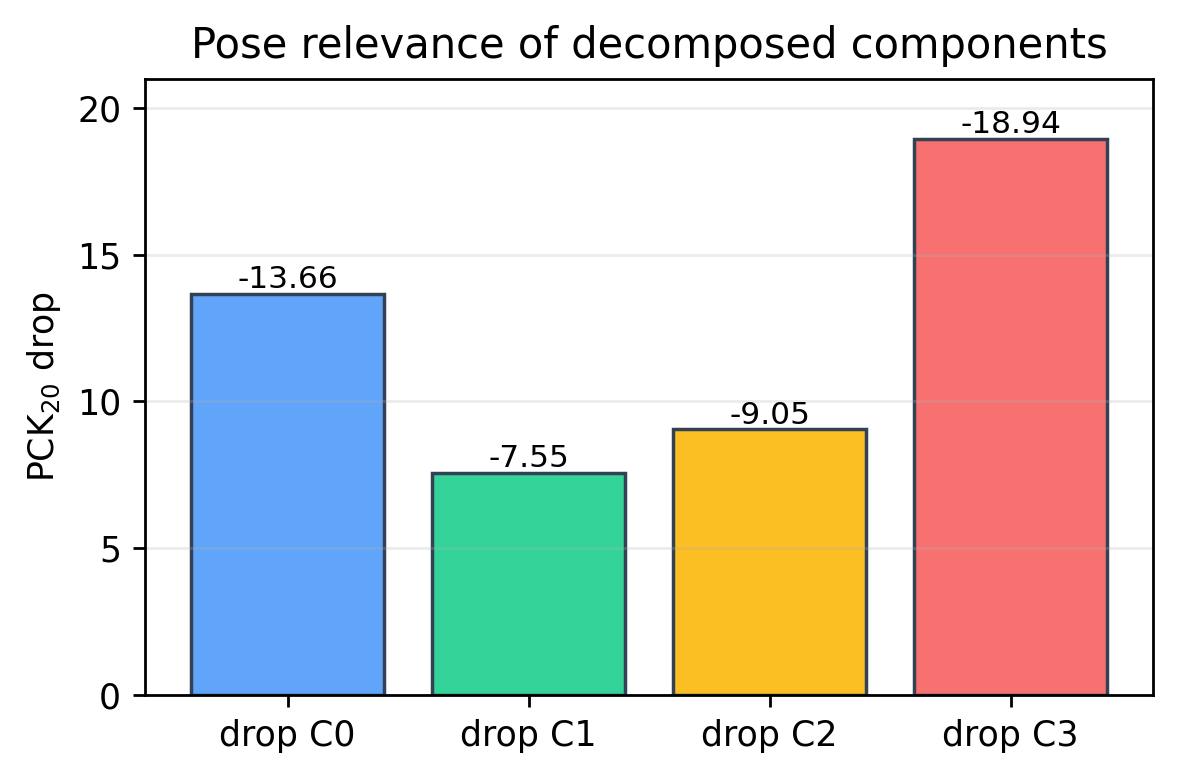
\includegraphics[width=\linewidth]{figures/fig3_component_ablation.pdf}
\caption{Component pose relevance. Removing any component reduces PCK$_{20}$, showing that the decomposition is not cosmetic.}
\label{fig:component_ablation}
\end{figure}

\begin{table}[t]
\centering
\caption{Component ablation with CP components + ExtraTrees.}
\label{tab:component}
\begin{tabular}{lrr}
\toprule
Input & PCK$_{20}$ & Drop \\
\midrule
All components & 50.40 & 0.00 \\
Drop component 0 & 36.74 & -13.66 \\
Drop component 1 & 42.85 & -7.55 \\
Drop component 2 & 41.35 & -9.05 \\
Drop component 3 & 31.46 & -18.94 \\
\bottomrule
\end{tabular}
\end{table}

\subsection{Which Physical Mode Matters?}

We next remove entire factor modes. Figure~\ref{fig:factor_importance} shows that the subcarrier factor $B$ dominates the current frame-level setting. Removing $B$ causes a 24.90-point PCK$_{20}$ drop, while removing link factor $A$ causes a 2.68-point drop and removing packet factor $C$ causes only a 0.26-point drop. This is physically plausible: each MM-Fi frame contains only 10 packets, so within-frame temporal evidence is limited, while the 114-subcarrier axis captures frequency-selective multipath structure shaped by body geometry.

\begin{figure}[t]
\centering
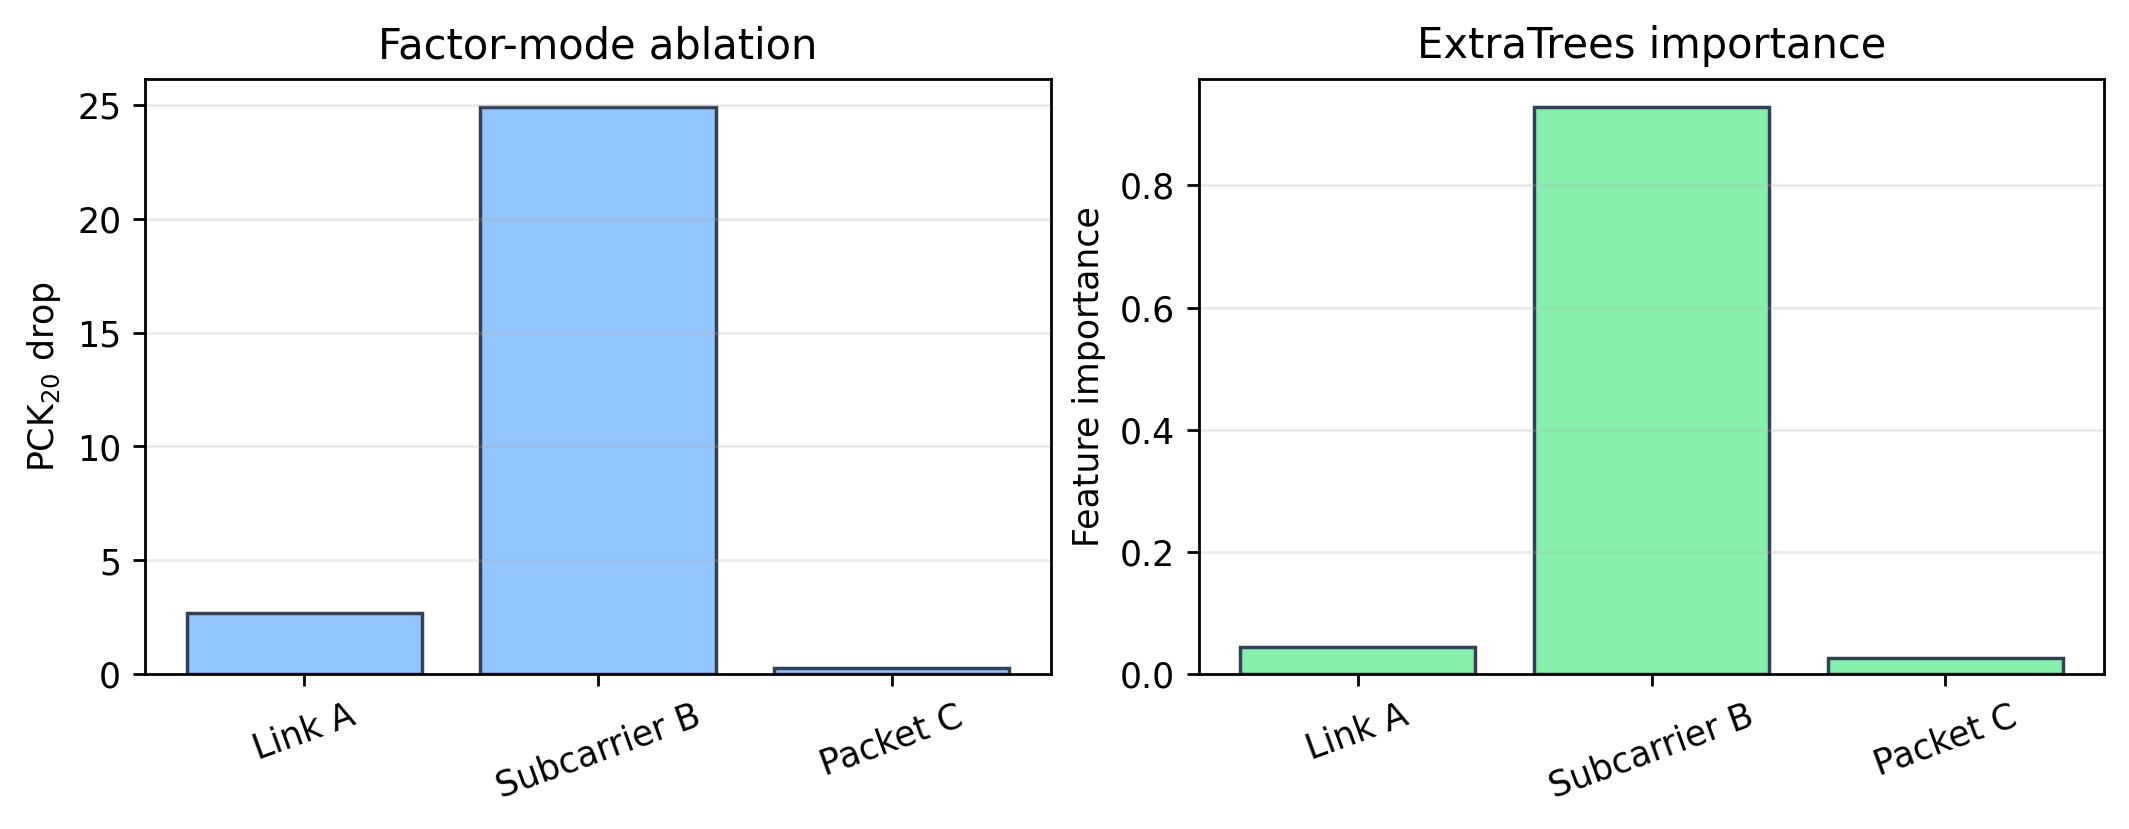
\includegraphics[width=\linewidth]{figures/fig4_factor_importance.pdf}
\caption{Factor-mode analysis. Under single-frame MM-Fi, the subcarrier factor carries most pose-relevant information.}
\label{fig:factor_importance}
\end{figure}

\subsection{Efficiency}

\begin{table}[t]
\centering
\caption{Model complexity of lightweight \method\ variants. FLOPs include CP feature extraction and pose regression.}
\label{tab:complexity}
\begin{tabular}{lrrrr}
\toprule
Model & Params & CP iters & MACs & FLOPs \\
\midrule
CP+Ridge & 25.9K & 5 & 0.259M & 0.518M \\
CP+MLP64 & 35.9K & 5 & 0.269M & 0.538M \\
CP+Ridge & 25.9K & 10 & 0.492M & 0.984M \\
CP+MLP64 & 35.9K & 10 & 0.502M & 1.004M \\
CP+AFF & 44.3K & 10 & 1.423M & 2.846M \\
CP+CNN & 77.6K & 10 & 2.530M & 5.059M \\
CP+Ridge & 25.9K & 35 & 1.658M & 3.316M \\
CP+MLP64 & 35.9K & 35 & 1.668M & 3.336M \\
\bottomrule
\end{tabular}
\end{table}

Compared with HPE-Li's reported 1.66M parameters and 2.42G FLOPs, CP+AFF uses about 37$\times$ fewer parameters and over 850$\times$ fewer FLOPs. CP+MLP64 is even smaller, but AFF provides a better accuracy-efficiency balance. CP+CNN improves accuracy further but doubles the AFF compute. Therefore, the practical deployment story is CP+AFF: it is small enough for real devices, structured enough to exploit decomposed factors, and accurate enough to approach neural HPE baselines.

\section{Discussion}

\textbf{What the current evidence proves.}
The full-MM-Fi results show that decomposed CSI components are compact, predictive, and pose-relevant. They improve lightweight nonlinear predictors over raw statistics and enable a much smaller model than HPE-Li. The ablation evidence is strong: removing components or the subcarrier factor sharply degrades PCK.

\textbf{What it does not yet prove.}
We do not claim that vanilla CP is the final answer or that it cleanly separates physical human-motion sources. Vanilla CP is unsupervised and optimized only for reconstruction. Its factors are useful, but not necessarily maximally discriminative or physically pure.

\textbf{Next step: pose-aware decomposition.}
The natural next model is supervised or constrained decomposition using Eq.~\ref{eq:general_objective}. Diversity can reduce redundant components, sparsity can sharpen physical support, smoothness can stabilize temporal factors, and pose supervision can make factors more keypoint-relevant. This would turn \method\ from a decomposition-first proof of concept into a stronger SOTA competitor.

\textbf{Hardware deployment.}
The compute numbers suggest that CP+AFF is suitable for Raspberry Pi and Jetson Nano deployment. Unlike ExtraTrees, AFF consists of dense layers, lightweight convolutions, and a softmax gate, making it friendly to standard neural runtimes such as TorchScript, ONNX Runtime, TensorRT, or vendor-optimized CPU kernels. The final paper should include measured latency, memory, power, and FPS on real devices. Since the predictor is tiny, the main hardware bottleneck will likely be decomposition extraction. This motivates either optimized CP kernels or a learned feed-forward factor extractor.

\section{Conclusion}

This paper introduces \method, a decomposition-first framework for Wi-Fi human pose estimation with component-adaptive fusion. Instead of forcing a neural network to infer pose directly from entangled CSI, \method\ first factorizes CSI into compact link, subcarrier, and packet components, then uses AFF to fuse these physical factors with a tiny deployment-friendly neural predictor. On full MM-Fi protocol3, CP components improve lightweight nonlinear predictors over raw-statistic features and show strong pose relevance under ablation. CP+AFF reaches a practical middle point: substantially smaller and cheaper than HPE-Li, more accurate than ultra-tiny MLP64, and easier to deploy than tree ensembles. These findings support a broader research direction: build Wi-Fi HPE systems around interpretable signal decomposition and hardware-friendly component fusion.

\bibliographystyle{aaai}
\begin{thebibliography}{99}

\bibitem{personwifi2019}
F. Wang et al.
\newblock Person-in-WiFi: Fine-grained person perception using WiFi.
\newblock arXiv:1904.00276, 2019.

\bibitem{wimose2020}
Y. Wang et al.
\newblock Wi-Mose: 3D moving human pose estimation using commodity WiFi.
\newblock arXiv:2012.14066, 2020.

\bibitem{gopose2022}
J. Geng et al.
\newblock GoPose: 3D human pose estimation using WiFi.
\newblock arXiv:2204.07878, 2022.

\bibitem{metafi2022}
Z. Zhao et al.
\newblock MetaFi: Device-free pose estimation via commodity WiFi.
\newblock arXiv:2208.10414, 2022.

\bibitem{mmfi2023}
Y. Yang et al.
\newblock MM-Fi: Multi-modal non-intrusive 4D human dataset for versatile wireless sensing.
\newblock arXiv:2305.10345, 2023.

\bibitem{hpeli2024}
T. D. Gian et al.
\newblock HPE-Li: WiFi-enabled lightweight dual selective kernel convolution for human pose estimation.
\newblock ECCV, 2024.

\bibitem{widefus2026}
W. Liu et al.
\newblock WiDeFus: A Wi-Fi-based lightweight human activity recognition via CSI component decomposition and adaptive feature fusion.
\newblock IEEE Transactions on Cognitive Communications and Networking, 2026.

\bibitem{kolda2009}
T. G. Kolda and B. W. Bader.
\newblock Tensor decompositions and applications.
\newblock SIAM Review, 2009.

\bibitem{lee1999}
D. D. Lee and H. S. Seung.
\newblock Learning the parts of objects by non-negative matrix factorization.
\newblock Nature, 1999.

\bibitem{graphposefi2025}
Anonymous.
\newblock GraphPose-Fi: Graph-based Wi-Fi human pose estimation.
\newblock arXiv:2511.19105, 2025.

\bibitem{cmambapose2026}
Anonymous.
\newblock C-MambaPose: A physics-informed complex Mamba framework for cross-environment WiFi human pose estimation.
\newblock arXiv:2606.13700, 2026.

\end{thebibliography}

\end{document}
